% !TEX root = ../linal_lecture_06.tex

\begin{frame} % название фрагмента

\videotitle{Обобщение диагонализации}

\end{frame}



\begin{frame}{Краткий план:}
  \begin{itemize}[<+->]
    \item Жорданова нормальная форма.
    \item Сингулярное разложение.
    \item Доказательство существования.
  \end{itemize}

\end{frame}


\begin{frame}
  \frametitle{Не все матрицы диагонализуемы}

  \begin{block}{Утверждение}
    Квадратная матрица $A$ размера $n\times n$ диагонализуема, если у неё найдётся $n$ линейно независимых собственных векторов.

    В этом случае $A$ представима в виде $A  =  P D P^{-1}$,

    где $P$ — матрица из собственных векторов, $D$ — диагональная матрица из собственных значений. \pause
  \end{block}

  \begin{block}{Утверждение}
    У симметричной матрицы $A$ размера $n\times n$ найдётся $n$ ортогональных собственных векторов единичной длины.

    С их помощью матрица $A$ представима в виде
    \[
    A = P D P^T.      
    \]
  \end{block}


\end{frame}


\begin{frame}
  \frametitle{А если не везёт?}

  Что делать, если у матрицы $A$ размера $n\times n$ меньше, чем $n$ независимых
  собственных векторов? \pause
  
  
  \begin{block}{Утверждение}
  Любая квадратная матрица $A$ представима в виде
  \[
  A = P J P^{-1},  
  \]
  где \alert{жорданова нормальная форма} $J$ содержит на диагонали \alert{жордановы клетки} $J_i$:
  \[
  J = \begin{pmatrix}
    J_1 & \bzero & \ldots & \bzero \\
    \bzero & J_2 & \ldots & \bzero \\
    \ldots & \ldots & \ldots & \bzero \\
    \bzero & \bzero & \ldots & J_k \\
  \end{pmatrix}, \quad
  J_i = \begin{pmatrix}
\lambda_i & 1 & \ldots & 0 \\
0 & \lambda_i & \ldots & 0 \\
0 & \ldots & \ldots & 1 \\
0 & 0 & \ldots & \lambda_i \\    
  \end{pmatrix}
  \]
  \end{block}

\end{frame}



% \begin{frame}
%   \frametitle{Жорданова нормальная форма}

%   \begin{block}{Алгоритм}
%     \begin{enumerate}
%       Для каждого собственного числа $\lambda$ матрицы $A$:

%       \item Находим максимальное количество независимых собственных векторов
%       с собственным числом $\lambda$.

%       Обозначим это множество $LI_\lambda = \{\ba, \bb, \bc, \ldots \}$. \pause


%       Количество векторов в  $LI_\lambda$ равно числу жордановых клеток с данным $\lambda$. \pause


%       \item Для собственного вектора $\bv \in LI_\lambda$ находим последовательно
%       \alert{присоединённые векторы}, решая цепочку линейных уравнений:
      
%       \[
%       \begin{array}{l}
%         (A - \lambda \Id) \bv_1 = \bv \\
%         (A - \lambda \Id) \bv_2 = \bv_1 \\
%         (A - \lambda \Id) \bv_3 = \bv_2 \\
%         \ldots 
%       \end{array}
%       \]

%     \end{enumerate}
    
%   \end{block}

% \end{frame}


\begin{frame}
  \frametitle{Сингулярное разложение}

  \begin{block}{Утверждение}
    Любой линейный оператор из $\R^k$ в $\R^n$ представляет собой последовательность действий: \pause

    \begin{enumerate}
      \item Ортогональное преобразование из $\R^k$ в $\R^k$. Сохраняет длины векторов и углы между ними. \pause
      \item Растягивание компонент вектора в $\R^k$. \pause
      \item Переход из $\R^k$ в $\R^n$ путём дописывания нулей в вектор, или зачёркивания части координат. \pause
      \item Ортогональное преобразование из $\R^n$ в $\R^n$. Сохраняет длины векторов и углы между ними. \pause
    \end{enumerate}  
  \end{block}

  Все эти действия мы рассмотрели на первой лекции!

\end{frame}


\begin{frame}
  \frametitle{Сингулярное разложение проекции}

  Оператор $\HH: \R^n \to \R^n$ проецирует векторы на линейную оболочку $M$. \pause

  Выберем ортогональный базис $\bv_1$, $\bv_2$, \ldots, $\bv_k$ в $M$. \pause

  Дополним его до ортогонального базиса в $\R^n$ векторами $\bv_{k+1}$, \ldots, $\bv_n$. \pause


  \begin{enumerate}
    \item Повернём-отразим пространство, чтобы $\bv_1$, \ldots, $\bv_n$ перешли в $\be_1$, \ldots, $\be_n$. \pause
    \item Домножим первые $k$ компонент вектора на 1, а остальные на 0.  \pause
    \item Смены размерности нет. \pause
   \item Повернём-отразим пространство, чтобы $\be_1$, \ldots, $\be_n$ перешли в $\bv_1$, \ldots, $\bv_n$. 
  \end{enumerate}  

\end{frame}



\begin{frame}
  \frametitle{Сингулярное разложение}

  \begin{block}{Утверждение}
    Любую матрицу $A$ размера $n\times k$ можно представить в виде
    \[
    A = U \Sigma V^T,  
    \]
    где матрица $U$ размера $n\times n$ — ортогональная, $U^TU=\Id$,

    матрица $V$ размера $k\times k$ — ортогональная, $V^TV=\Id$,

    матрица $\Sigma$ размера $n\times k$ — диагональная.
    
  \end{block} \pause

  Данное разложение также называется \alert{$SVD$-разложением}, singular value decomposition.

\end{frame}
  



\begin{frame}
  \frametitle{Присмотримся к матрицам}

  Если $n\geq k$, то $SVD$-разложение примет вид

  \[
  A = \begin{pmatrix}
    \vert &  & \vert \\
    \bu_1 & \ldots & \bu_n \\
    \vert &    & \vert \\
  \end{pmatrix} \cdot 
  \begin{pmatrix}
    \sigma_1 & 0 & \ldots & 0 \\
     0 & \sigma_2 & \ldots & 0 \\
    \ldots & \ldots & \ldots & \ldots \\
0 & 0 & \ldots & \sigma_k \\
0 & 0 & \ldots & 0 \\
\ldots & \ldots & \ldots & \ldots \\
0 & 0 & \ldots & 0 \\
  \end{pmatrix} \begin{pmatrix}
\text{—}  \hspace{-0.2cm} & \bv_1^T & \hspace{-0.2cm}  \text{—} \\
 & \vdots &  \\
\text{—}  \hspace{-0.2cm} & \bv_k^T & \hspace{-0.2cm}  \text{—} \\
   \end{pmatrix} \pause
  \]

  Числа $\sigma_i$ называются \alert{сингулярными} числами матрицы $A$.
  
\end{frame}


\begin{frame}
  \frametitle{Зачем нужно $SVD$-разложение?}

  Сильно упрощает многие вычисления.  \pause

  Показывает внутренний мир матрицы. \pause

  Существует быстрая и устойчивая итеративная процедура нахождения $SVD$-разложения. 

\end{frame}

\begin{frame}
  \frametitle{Раскладываем все матрицы!}
  
  Сингулярное разложение для $A^T$:
  \[
  A^T = (U\Sigma V^T)^T = V \Sigma^T U^T   \pause
  \]
  Сингулярное разложение для $A^TA$:
  \[
  A^TA = V \Sigma^T U^T \cdot U\Sigma V^T = V \Sigma^T\Sigma V^T  \pause
  \]
  Сингулярное разложение для $AA^T$:
  \[
  AA^T = U\Sigma V^T \cdot  V \Sigma^T U^T =  U \Sigma \Sigma^T U^T 
  \]

\end{frame}


\begin{frame}
  \frametitle{Существование разложения}

  Наша задача предъявить разложение $A = U\Sigma V^T$.
  
  Для удобства будем считать, что $n \geq k$. \pause


  \begin{block}{Доказательство}
    \begin{enumerate}
      \item Матрица $A^TA$ является матрицей Грама. Она положительно определена и симметрична.
      А потому представима в виде $A^TA = V D V^T$. \pause

      \item Диагональные элементы $D$ неотрицательны. Поэтому $D$ представима 
      в виде $\Sigma^T \Sigma$. \pause

      \item Осталось найти $U$ из целевого разложения:
      \[
        A = U\Sigma V^T\pause \text{ или } AV = U\Sigma  
      \]
\end{enumerate}


\end{block}

\end{frame}

\begin{frame}
\frametitle{Существование разложения}

Уже нашли $\Sigma$ и $V$. Осталось найти $U$ из $AV = U\Sigma$. \pause

\begin{block}{Окончание доказательства}
\begin{enumerate}

      \item[4.] Находим вектора $\bu_i$ по очереди:
      \[
        \bu_1 = A\bv_1 / \sigma_1, \pause \; \bu_2 = A\bv_2 / \sigma_2, \ldots \pause
      \]
      \item[5.] Вектора $\bv_i$ кончатся раньше $\bu_i$. \pause
      Оставшиеся $\bu_{k+1}$, \ldots, $\bu_{n}$ выберем произвольными, чтобы $U$ была ортогональной матрицей.

\end{enumerate}
\end{block}

  

\end{frame}



\begin{frame}
 \frametitle{Авторы современного алгоритма}


	
	
\begin{figure}[H]
  \noindent\makebox[\textwidth][c]{%
    \begin{minipage}[H]{0.5\linewidth}
      \begin{figure}
      \centering
        \caption{Джин Говард Голуб}
        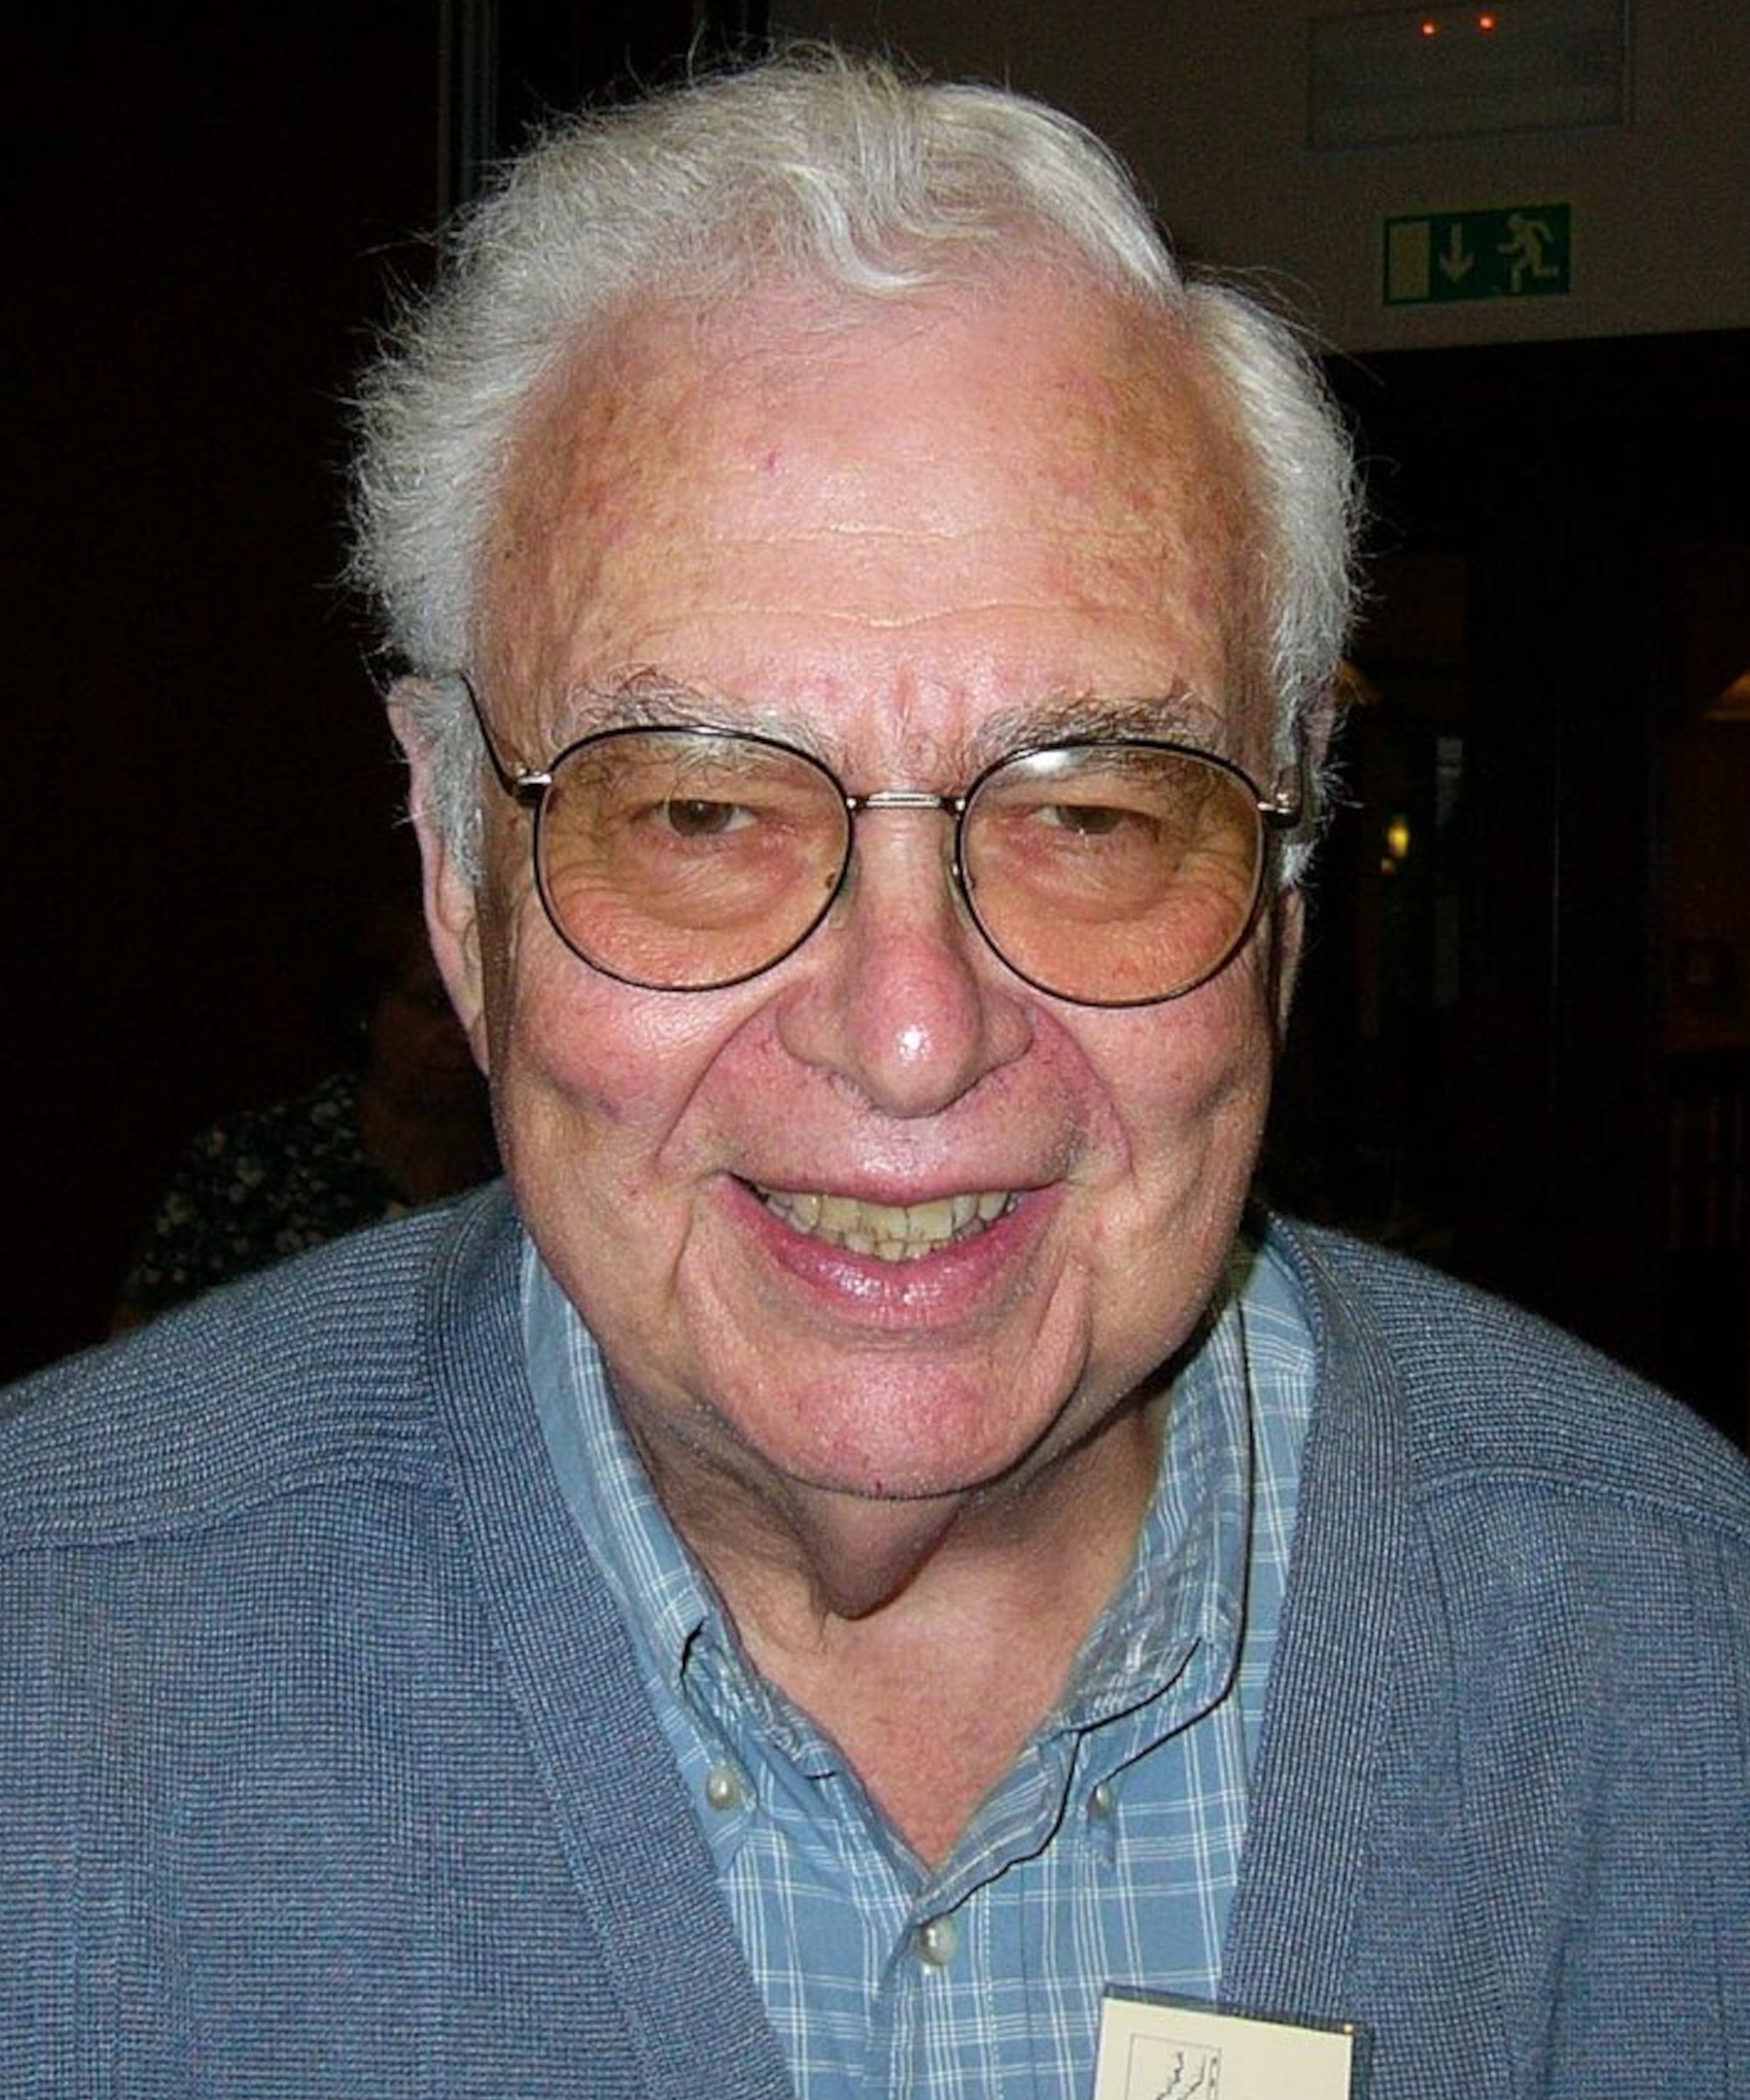
\includegraphics[width=0.7\linewidth]{figures/pic_genegolub}
        \label{fig:picgenegolub}
      \end{figure}
    \end{minipage}
    \begin{minipage}[H]{0.5\linewidth}
      \begin{figure}
        \centering
        \caption{Уильям Мортон Кэхэн}
        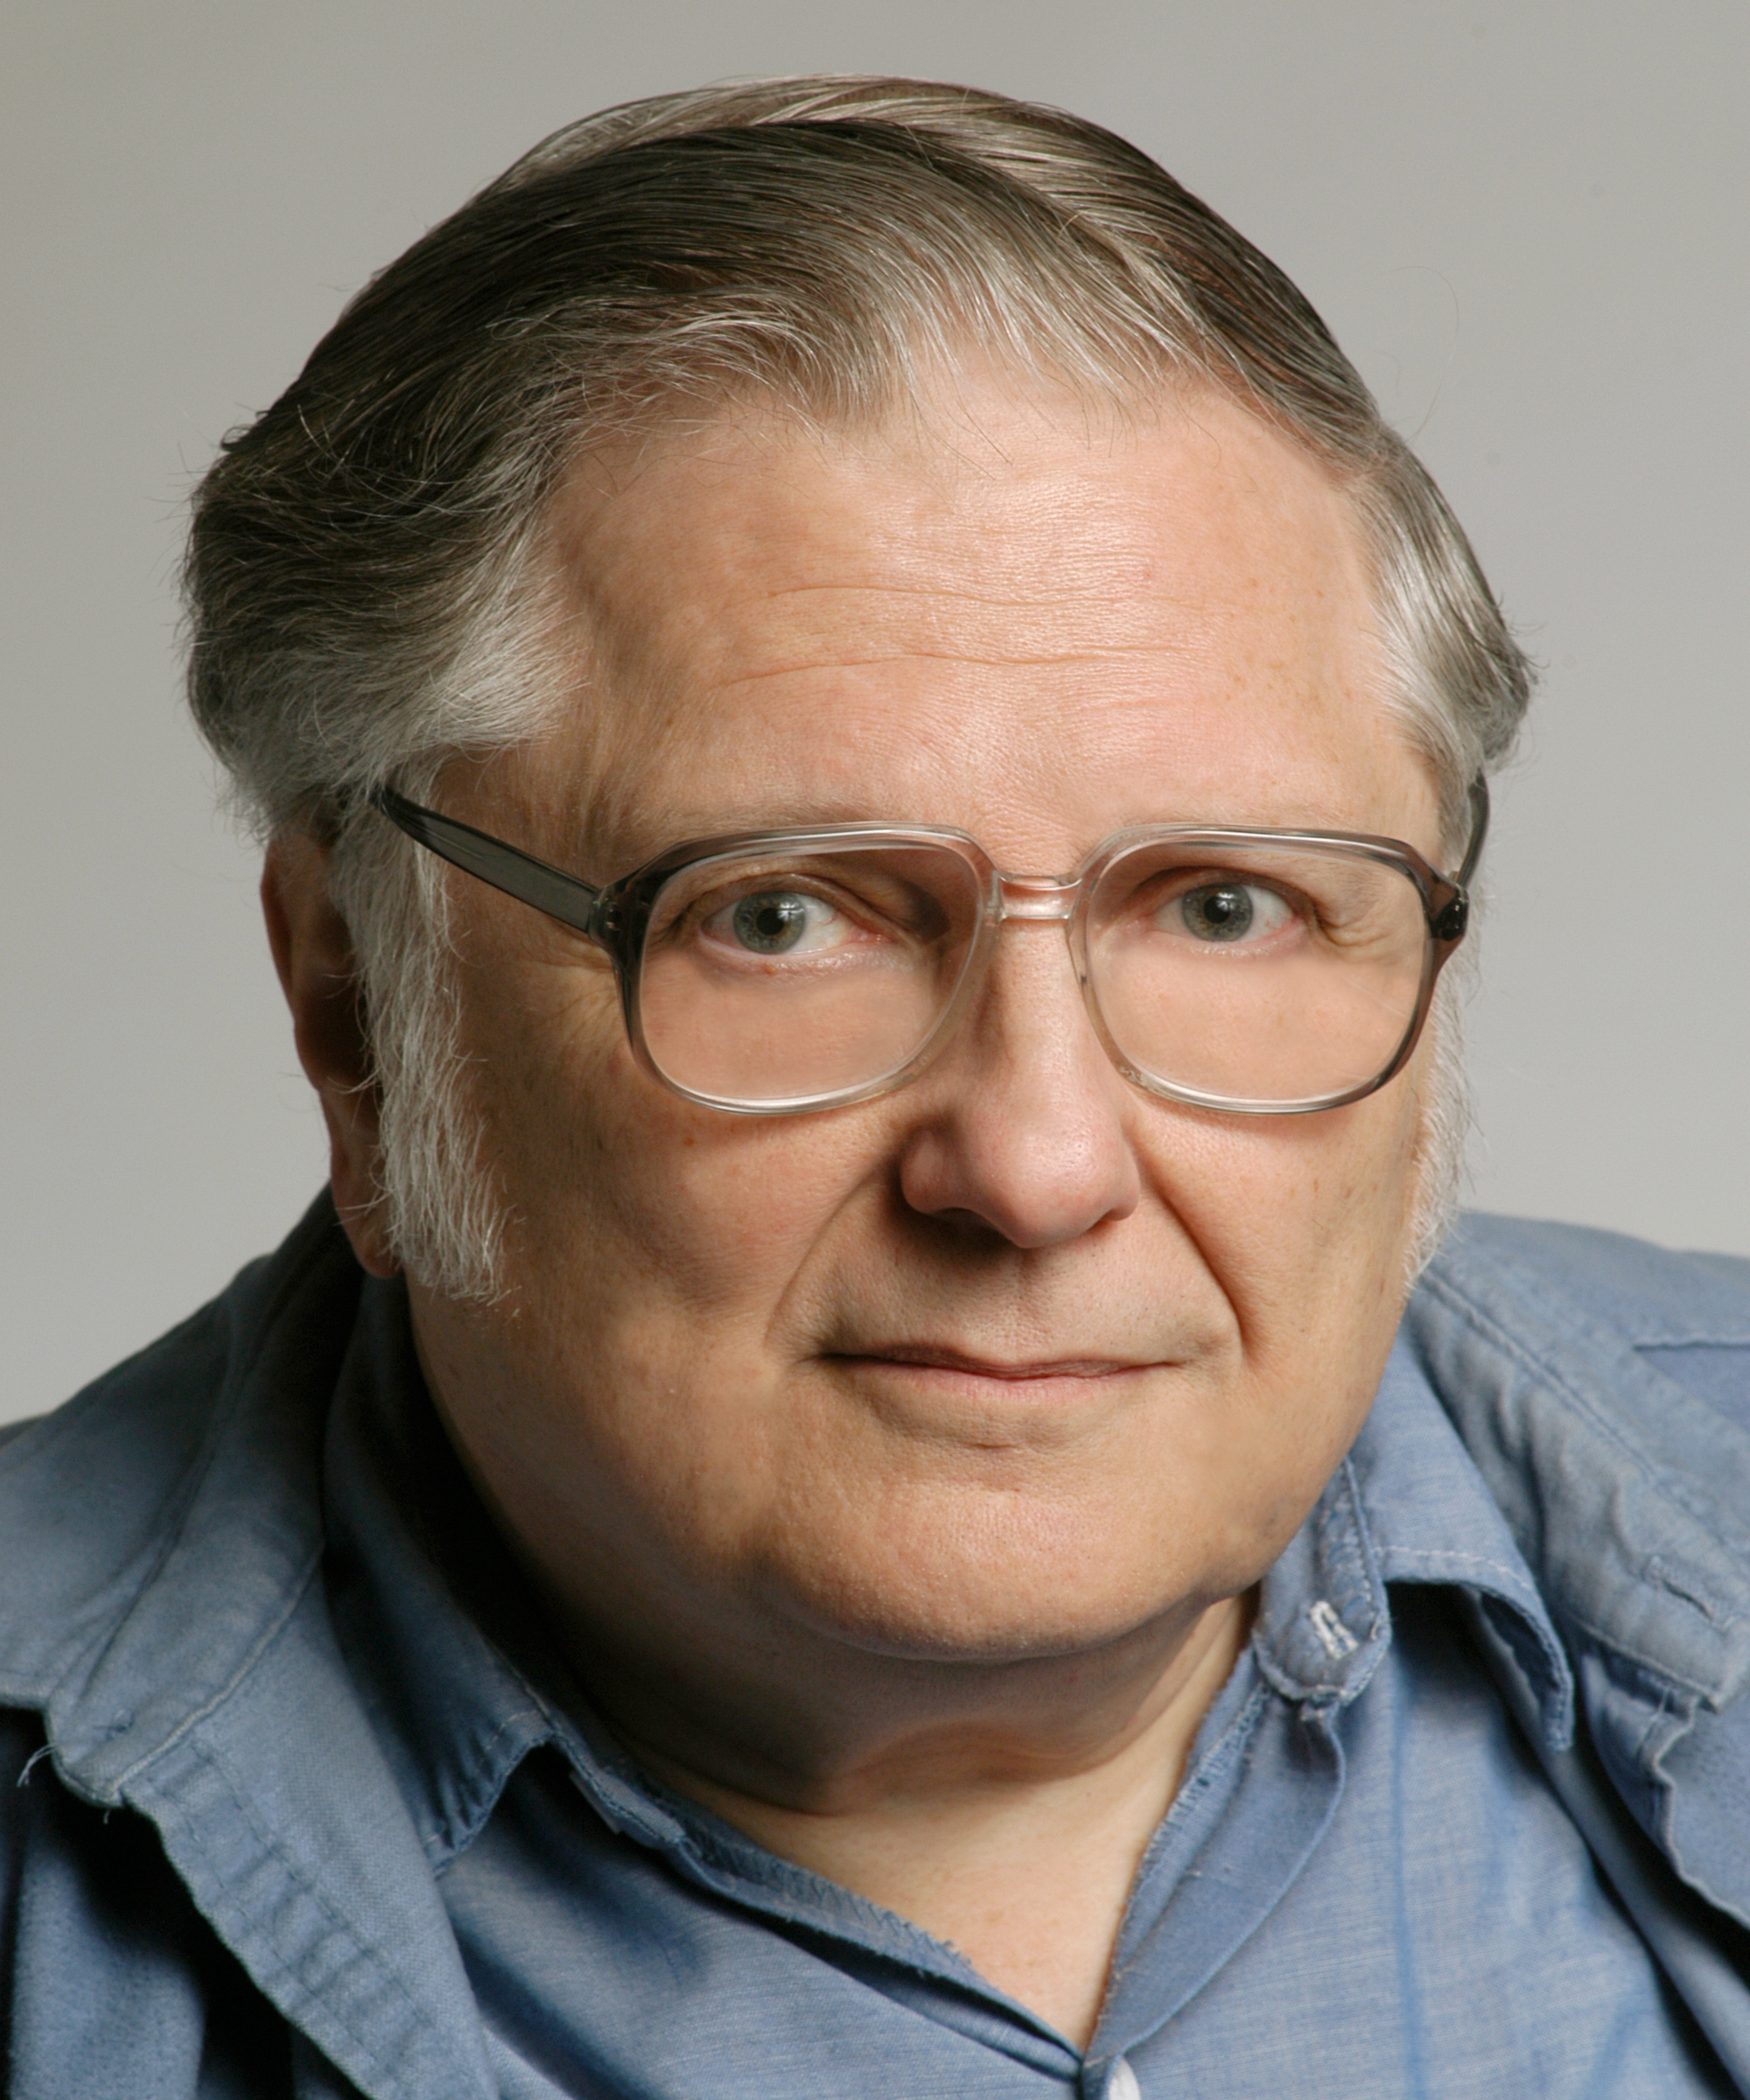
\includegraphics[width=0.7\linewidth]{figures/pic_kahan}
        \label{fig:pickahan}
      \end{figure}
    \end{minipage}
    \hfill
  }
\end{figure}

\begin{figure}[H]
\noindent\makebox[\textwidth][c]{%
  \begin{minipage}[H]{0.5\linewidth}
    \begin{figure}
      \centering
      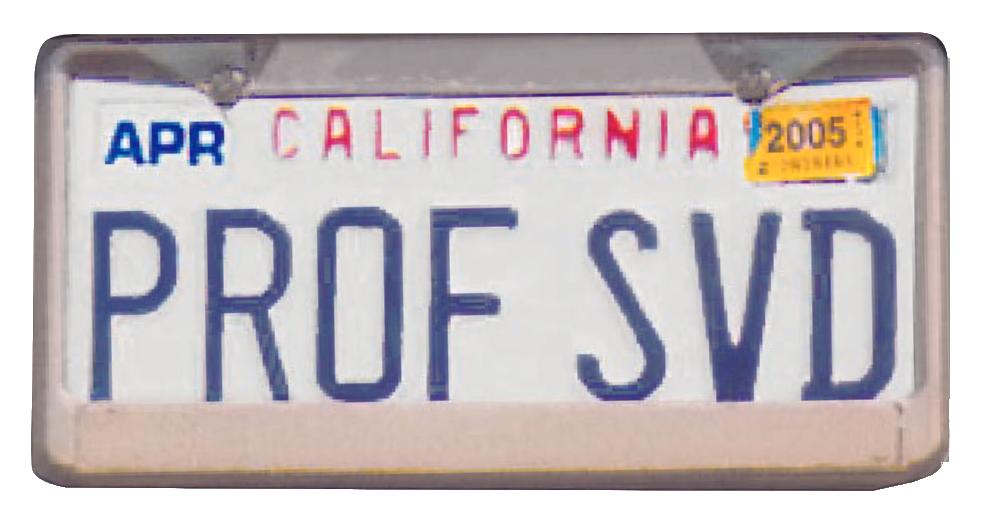
\includegraphics[width=0.5\linewidth]{figures/pic_plate}
%				\caption{}
      \label{fig:picplate}
    \end{figure}
  \end{minipage}
  \begin{minipage}[H]{0.5\linewidth}
\hspace{35pt}Отец плавающей точки
  \end{minipage}
  \hfill
}
\end{figure}



\graylink{wikipedia.org / П. Биркен, Д. Биркен, фото номера: П.М. Кроненберг, Клив Молер}



\end{frame}
